% Copyright (c) 2017 Peter A. Audano III
% GNU Free Documentation License Version 1.3 or later
% See the file COPYING.DOC for copying conditions.

\section{The Kestrel Process}
\label{sec.process}

Kestrel is a different class of variant caller, and understanding how it works is the key to tuning it for your application.

\subsection{Overview}
\label{sec.process.overview}

\begin{figure}[H]
	
	\begin{center}
		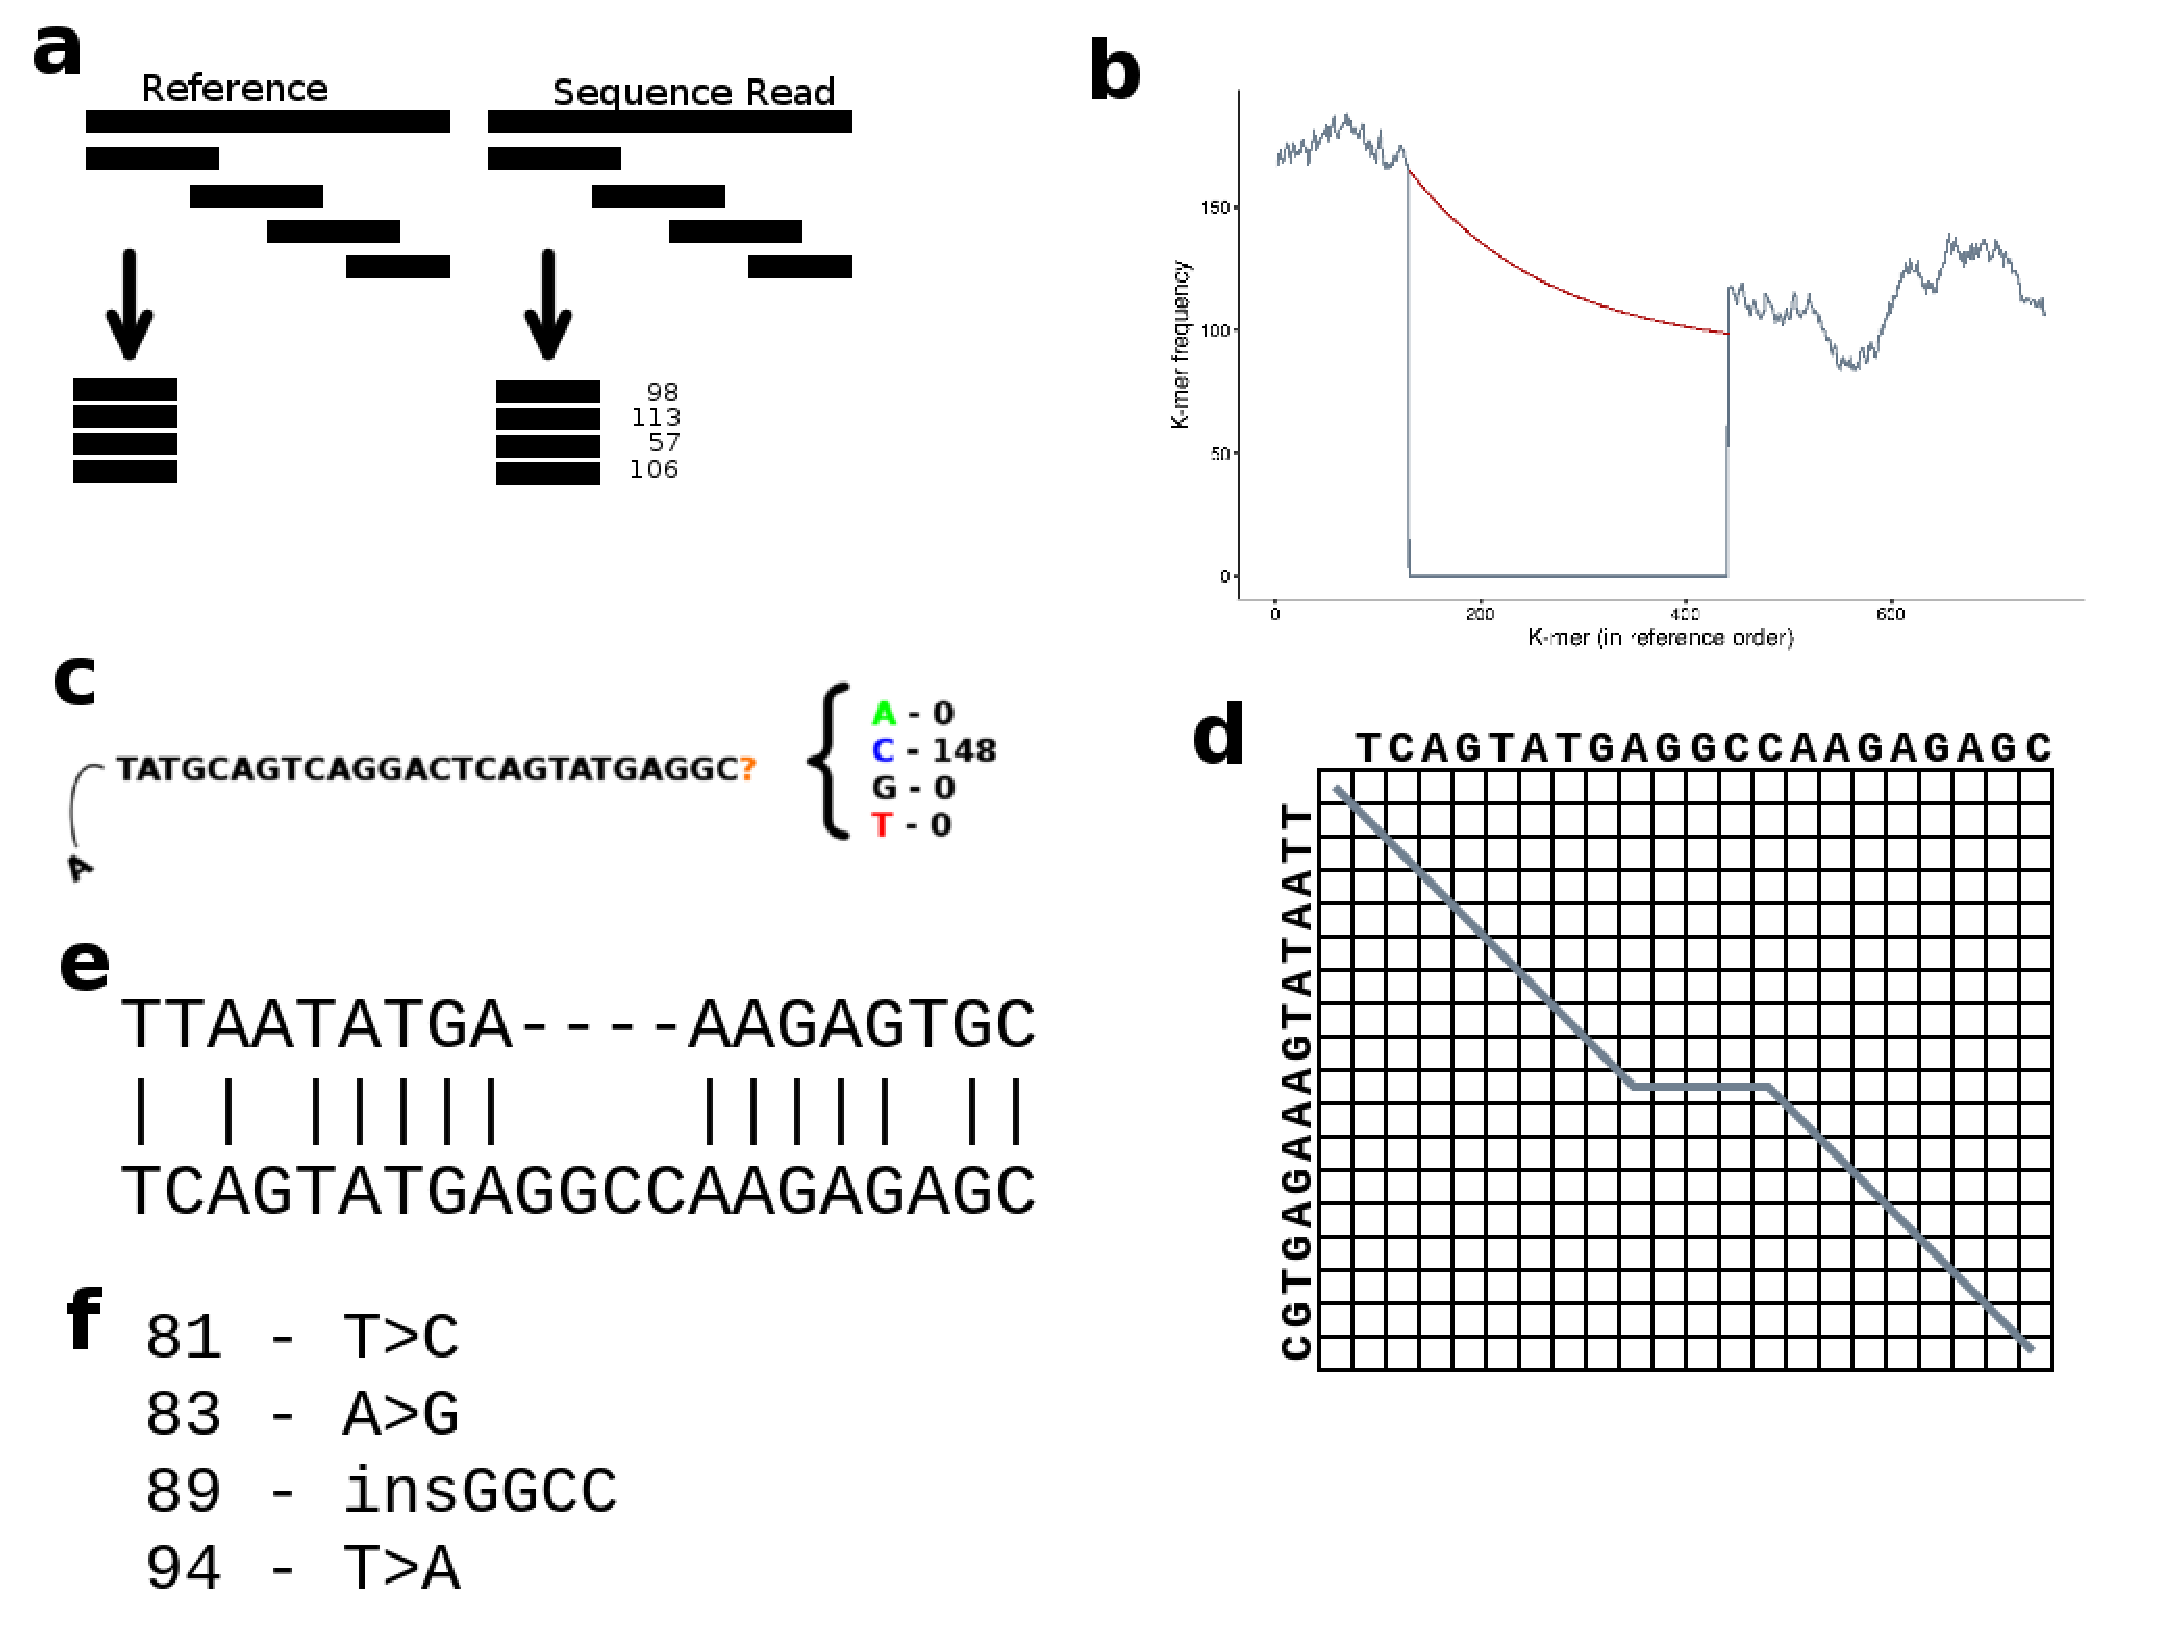
\includegraphics[width=0.75\textwidth]{img/KestrelOverview}
	\end{center}
	
	\caption{Overview of the Kestrel process from sequence data to variant call. \figpart{a} The reference sequence and the sequence reads are converted to k-mers. The k-mers of the sequence reads are counted, but the k-mers of the reference are left in order. \figpart{b} K-mer frequencies from the sequence reads (vertical axis) are assigned to the k-mers of the reference (horizontal axis). A decline and recovery of the frequencies bound an active region where one or more variants are present. \figpart{c} Starting from the left anchor k-mer (last k-mer with a high frequency), the first base is removed, each possible base is appended, and the base that recovers the k-mer frequency is appended to the haplotype. \figpart{d} A modified alignment algorithm tracks haplotype reconstruction and terminates the process when an optimal alignment is reached. \figpart{e} This algorithm yields an alignment of the reference sequence and haplotype within the active region. \figpart{f} Variant calls are extracted from the alignment.}
	
	\label{fig.arillustration}
\end{figure}

Kestrel first translates the reference sequence to a set of ordered k-mers and the sequence reads to k-mer frequencies. The frequency of each reference k-mer and its reverse-complement are queried and examined. The expected distribution of reference k-mer frequencies in a given region is roughly uniform. However, when a variant occurs, the k-mers of the sequence reads differs from the k-mers of the reference, and clear disruptions of the uniform distribution can be observed. For example, a single SNP will change $k$ k-mers, and the frequency of those reference k-mers will be much lower than those around it.

Kestrel scans the list of frequencies from the reference k-mers from left to right searching for regions where it declines sharply and recovers at some downstream k-mer. This region is an \textit{active region} where one or more variants are suspected to be found. The algorithm includes the high-frequency k-mers at either end of the active region, and these are called \textit{anchor k-mers} because the help to seed the process of resolving the region.

Kestrel then builds one or more local assemblies through the active region, and each one is called a \textit{haplotype}. Haplotype reconstruction begins on the left anchor k-mer, and since that k-mer is part of the active region, it is the first $k$ bases of the haplotype. According to active region detection, then next k-mer downstream should be altered, and this fact is used to simplify the process of resolving altered bases using an iterative sliding process.

Starting from the anchor k-mer, the first base is removed, each possible base (A, C, G, and T) are appended to the $(k - 1)$-mer, and the frequency of each possibility is checked. The reverese-complement k-mer is subjected to a similar process, and the frequencies are summed. The base that produces a k-mer with the highest frequency is appended to the haplotype. This process is repeated until the haplotype is fully resolved.

There are a couple of notable exceptions to the the process as described, and these will be covered in more detail. When more than one base produces a k-mer with an acceptable frequency, haplotype reconstruction splits by saving one of the possibilities, building the most likely one, and returning to the other saved states. If a variant occurs too close to the start of a reference, Kestrel can start from the right anchor k-mer and work backwards. In this case, the left anchor k-mer is missing, and a Kestrel option must be used to allow only one anchor.

Kestrel uses a modified Smith-Waterman~\cite{Smith1981} alignment to guide haplotype reconstruction over the active region. When an optimal alignment score is reached, haplotype reconstruction terminates. An additional check ensures that the active region ends on the right anchor k-mer or the haplotype is discarded. If only one haplotype is found and it matches the reference, it is discarded and Kestrel omits nothing for that region.

The alignment of each haplotype over an active region is then used to find variants. Kestrel sums the evidence for the variant from each haplotype it is found in.


\subsection{Input}
\label{sec.process.input}

\subsubsection{Sequence Data}
\label{sec.process.input.seq}
Because Kestrel relies on the KAnalyze~\cite{Audano2014} API for its sequence input, it can take any file format KAnalyze can read. This includes FASTA, FASTQ, gzipped FASTA and FASTQ, and indexed k-mer count (IKC). Kestrel uses the KAnalyze stream mode to convert the reference to an ordered list of k-mers.

\lopt{format} can be used be to force the input file format for all files following it on the command line. The default value, ``auto'', attempts to determine the input file format by the file name. This is handled by KAnalyze, and so Kestrel can input anything KAnalyze can turn into an IKC file. \lopt{stdin} can be used in place of an input file, and Kestrel will read sequence data from standard input.

Sequence data can be filtered before it is turned into k-mers. The options \lopt{seqfilter} and \lopt{quality} are synonymous and equivalent to the KAnalyze sequence filters. The format of the argument to this option is ``FILTER:ARGS'', where FILTER is the filter name, and ARGS is a string of arguments. The format of the arguments is up to the filter, but it is typically a comma-separated string of attributes and values. The default filter is ``sanger'', which applies a quality filter assuming Sanger FASTQ quality scores (Phred scaled). This filter can take a numeric value specifying the minimum score. This option applied the filter to all subsequent input files, but \lopt{noseqfilter} may be used to turn it off so that the filter is not applied to all input.

\subsubsection{Reference}
\label{sec.process.input.seq}

The reference file is input with \lopt{ref}, and this option may be used multiple times if reference sequence is found in multiple files. Reference files are also processed by KAnalyze, and they can be in any format KAnalyze can stream k-mers from (not IKC). The reference does not need to be indexed in any way.

The description line of a FAST record has a sequence identifier with an optional extended description. KAnalyze assumes everything after the first whitespace character is an extended description, and it is not part of the record ID. If whitespace characters are part of the the sequence name and should not be discarded, \lopt{normrefdesc} may be used to retain the description as part of the record ID.


\subsubsection{Samples}
\label{sec.process.input.samples}

Kestrel can call variants on multiple samples in one run, but by default, it assumes all input data belongs to the same sample. Any sample may have more than one file of sequence data in it. These files are read, translated to k-mers, counted, and stored in an IKC file. Any input except IKC file may be mixed into one sample, but if an IKC file is used, it must not be accompanied by any other sequence data including other IKC files.

If no sample names (\lopt{sample}) is given, then Kestrel chooses a name for the sample based on the first input file name. Each time \lopt{sample} is found, it starts a new sample and all subsequent files up to the next \lopt{sample} is grouped into one sample. Samples without any input files are ignored.

In some cases, it is more convenient to input a list of files and have Kestrel separate them automatically instead of repeated used of \lopt{sample}, and Kestrel provides \lopt{filespersample} to make this easier. For example, many samples of paired-end reads can be input by setting \lopt{filespersample} to $2$ and ensuring input files are paired on the command-line. Kestrel will use default names for samples. The default value, $0$, does no automatic grouping. \lopt{sample} will override \lopt{filespersample} and reset the number of files in the current sample if these options are mixed.

\subsection{K-mer Counting}
\label{sec.process.kmers}

The most important option for k-merization is the k-mer size, \lopt{ksize}. Larger k-mers are more specific, but are more likely to contain errors, and fewer k-mers can be extracted from sequence reads. A k-mer size too small is not specific enough, and a k-mer size too large leads to loss of coverage. The default, 31, is used for historical reasons, but k-mers up to size 48 have been used successfully with human data. Tune this parameter for read size and error rate.

Sequence read errors generate erroneous low-frequency k-mers, and \lopt{mincount} controls the minimum frequency. K-mers with a count less than this value will be discarded before being merged into the IKC. This keeps the IKC file to a reasonable size. During k-mer counting, however, all k-mers are written to a temporary location (\lopt{temploc}) before being merged, and the temporary files are automatically deleted.

Input sequence reads are converted to an IKC file. This file is a database of k-mers that can be rapidly searched without loading the k-mer counts into memory. It groups k-mers that likely appear together in a sequence, and when loaded as a memory-mapped file, segments of the file can be loaded as needed. The IKC file is automatically deleted by Kestrel when it is no longer needed, and this can be altered with \lopt{normikc}. KAnalyze can be used directly to generate the IKC in a separate step, and when Kestrel reads an existing IKC, it will never be automatically deleted.

If \lopt{memcount} is set, Kestrel will count k-mers to memory instead of an IKC file. It will be faster to query, but may use an excessive amount of memory.

The IKC format requires that k-mers be grouped by a minimizer, which is defined as the minimum value of all sub-k-mers of a k-mer and its reverse complement. Grouping by minimizers is the key to making IKC files fast without using much memory. The default, and maximum, minimizer size is 15. To better randomize k-mers over low-complexity sequence, minimizers may also be scrambled by an XOR mask by setting \lopt{minmask}. Changing these options is rarely necessary.

Active region detection, haplotype extension, and variant support all use the forward and reverse-complemented k-mers. If an application should strictly analyze and use evidence from a single strand, \lopt{nocountrev} may be set. In most cases, this option would only lower Kestrel's power to detect and resolve variants.

\subsection{Intervals and Flanks}
\label{sec.process.intervals}

Using a BED file specified by \lopt{interval}, Kestrel can call variants in specific regions of the genome. The BED file contains intervals over reference sequences (the first column must match reference sequence IDs).

If each region was treated as a reference sequence, then variants near the ends of the intervals may be lost. Kestrel can extend beyond the edges of these intervals, find active regions, and call variants from the extended interval. Any variants found outside of the actual interval are discarded after calling. By default, Kestrel extends intervals by $1.5 \cdot k$. This behavior can be controlled by \lopt{autoflank}, where a multiple of $k$ is set, or with \lopt{flank} with a set number of bases. Setting either of these options to $0$ will cause Kestrel to not use flanks.

Using intervals gives Kestrel a few output options as well. By default, Kestrel outputs variants relative to the start of the reference sequence, but \lopt{byregion} will output variants relative to the interval the variant was found in. If the BED file contains strand information, \lopt{revregion} may also be set to output variants relative to the positive strand (variants are complemented and shifted accordingly). These options are not recommended for VCF files as they will create a non-standard VCF that other tools and technicians may not know how to interpret correctly.


\subsection{Active Region Detection}
\label{sec.process.ardetect}

For each reference sequence or interval, Kestrel gets the k-mers in the order they appear. It then assigns the frequency from the IKC file to each of the k-mers. Variants between the sample and the reference change k-mers in the sample, and so the k-mers of the reference will have a lower frequency. These frequency disruptions appear as sudden dips followed by a recovery at some downstream k-mer. The active region is defined as the sequence covering these low-frequency k-mers, and it includes the high-frequency k-mers at each end.

\subsubsection{Scan Start}
\label{sec.process.ardetect.start}

The difference between neighboring k-mers must be large enough to trigger an active region scan, and this threshold is set dynamically by Kestrel. First, the difference between each pair of neighboring k-mers is found, and the threshold is set as a quantile of this difference distribution. The default quantile, 0.90, can be set with \lopt{diffq}. According to the default, 90\% of the differences between neighbors will be large enough to trigger an active region scan. This value is rather conservative, but it is limited by \lopt{mindiff} (default $5$), which sets the absolute minimum value this threshold can be regardless of the quantile.

\subsubsection{Scan End}
\label{sec.process.ardetect.end}

An active region scan ends when Kestrel finds an acceptable recovery of k-mer frequency at some downstream k-mer, but since sequence coverage is not uniform, Kestrel must allow for the possibility that the recovery k-mer frequency will be significantly lower than the anchor k-mer frequency where the scan started. Ideally, this threshold would start at the value of the left anchor k-mer and steadily decline to some minimum value as the scan moves further away. This function is defined as $f(x)$ where $x$ is the distance from the anchor k-mer and $f(0)$ is the anchor k-mer frequency.

$f(x)$ is based on a standard exponential decay function, $h(x) = e^{-x \lambda}$, which starts at $1$ and declines steadily toward $0$. $\lambda$ controls how fast it decays. $f(x)$ is defined by shifting $h(x)$ so that it approaches a minimum value, $f_{min}$, and scaled so that it declines from $f(x)$ to $f_{min}$.

Kestrel first determines the minimum value, $f_{min} = f(0) \cdot 0.55$, where the proportion of $f(0)$ can be set with \lopt{decaymin} (default 0.55). The exponential function is then scaled over the remaining distance from $f(0)$ to $f_{min}$ giving $f(x) = (f(0) - f_{min}) \cdot h(x) + f_{min}$.

The last parameter is $\lambda$, which is not set directly. Instead, $\lambda$ is determined by $\alpha$, which is defined as the proportion of $f(0) - f_{min}$ left after $k$ k-mers. The default value of $\alpha$ is $0.80$, and it can be set by \lopt{alpha}. This setting is far more intuitive than choosing some value of $\lambda$, and $\lambda$ can be readily found given $\alpha$ and $k$ (see Kestrel publication for details). Consequently, the range from $f(0) to f_{min}$ declined at $x$ is $x / k \cdot \alpha$. For example, when $X = 3k$, the recovery threshold is $\alpha^3 (f(0) \cdot f_{min}) + f_{min}$.

To summarize, an active region scan starts with anchor k-mer frequency $f(0)$. An exponential decay function is defined, $f(x)$, such that the recovery threshold declines steadily as the distance from the anchor k-mer, $x$, increases. When a k-mer $x$ k-mers away from the anchor is found with a frequency greater or equal to $f(x)$, the scan stops, and the k-mer at $x$ becomes the right anchor k-mer.

It is worth noting that stringently tuning $\alpha$ so that a scan ends at the end of an active region is not usually necessary. It is possible that the scan misses the end of an active region because the read depth declined too quickly. In this case, the active region scan will eventually decline to the read depth and stop. If other variants are nearby, the active region could start over one variant, miss the recovery, go into the next variant, and end when the k-mer frequency recovers. In this example, multiple variants will be covered in one active region, and Kesrel has no trouble with this.

\subsubsection{Resolving the Haplotypes}
\label{sec.process.ardetect.resolve}

When an active region scan successfully ends, the next step is to build haplotypes over it. The active region is then given over to the local assembly process of Kestrel. If at least one variant in the haplotypes exists, then they are output, and the search for the next active region begins after the right anchor k-mer.

If no haplotypes are resolved or if the only haplotype matches the reference, the active region is discarded and the search for the next active region starts from the first k-mer following the left anchor k-mer.

\subsubsection{Peak Detection}
\label{sec.process.ardetect.peak}

The sequence of a genome is not a random distribution of nucleotides. There are patterns, motifs, and duplicated regions, and these can be problematic for k-mer methods. While Kestrel cannot effectively deal with extended regions of homology, it can detect short peaks in the k-mer frequencies and ignore them. The maximum width of a peak in k-mers is set by \lopt{peakscan} (default = $7$). This value is used to avoid starting erroneous active region scans and to avoid prematurely ending active region scans.

When the k-mer frequency increases significantly, Kestrel first looks ahead to see if the frequency quickly declines again. If it does, it jumps ahead to the other side of the peak and continues to search for active regions.

When an active region scan finds a k-mer with a frequency meeting the recovery threshold, it looks ahead by the peak width to see if the frequency declines again, and if it does, it continues the scan from the other side of the peak as if the recovery threshold was not found.

It is possible that the active region scan will find many peaks at the end of an active region when the recovery threshold is very close to the read depth. When several peaks are found in quick succession, the active region scan goes back to the first sharp increase in frequency at the beginning of the peaks and ends there.

\subsubsection{Terminating a Scan}
\label{sec.process.ardetect.terminate}

Some active regions become so large that resolving them with Kestrel would use far too much memory and CPU to resolve, or they may be an erroneous active region. To limit the size of these regions, a limiting factor can be set. The active region limit is defined as the maximum length of a deletion, as calculated using the alignment weights, plus the k-mer size multiplied by $5.0$ (tunable with \lopt{scanlimitfactor}).

Active regions may span ambiguous bases, such as N. If, however, if \lopt{noambiregions} is set and the scan traverses an ambigous base, the active region is discarded.

If an active region reaches the end of the sequence, it cannot have both anchor k-mers and the scan is aborted. See \rsec{sec.process.ardetect.endcalling} for information about relaxing this limitation.

When a scan is terminated, the search for an active region continues from the next k-mer after what was the anchor k-mer in the active region scan.

\subsubsection{End Calling}
\label{sec.process.ardetect.endcalling}

If the active region does not have an anchor k-mer on both ends, it is also discarded by default. To enable calling variants up to the ends of reference sequences, \lopt{noanchorboth} can be set to allow a single anchor k-mer instead of requiring both. Calling to the ends is disabled by default because Kestrel could be extending a haplotype that actually belongs to another region. \lopt{noanchorboth} should be used with caution. For calling variants on intervals, Kestrel uses the flank options (\rsec{sec.process.intervals}) to avoid end-calling.

Kestrel can call variants up to either end of the reference. If a sharp increase of k-mer frequency is found before any other accepted active regions, it suggests that the beginning of the sequence may contain a variant affecting all k-mers at the start of the reference and the high-frequency k-mer is the \textit{right} anchor k-mer. Kestrel can then build from the right anchor k-mer in reverse to resolve variants up to the start of the sequence.

When a region lacks an anchor k-mer, Kestrel also allows deletions at the very ends. For all other regions with two anchor k-mers, end deletions are not allowed because the haplotypes must begin and end with the anchor k-mers.

\subsection{Haplotype Reconstruction}
\label{sec.process.haplo}

Haplotype reconstruction begins with the left anchor k-mer, and it extends to the right anchor k-mer. This process begins by assuming the left anchor k-mer matches the sequence and the haplotype, and so the haplotype sequence is initialized with the anchor k-mer sequence.

\subsubsection{Extending the Haplotype}
\label{sec.process.haplo.extend}

The haplotype is then extended by shifting the k-mer by one base into the active region. This is accomplished by taking the anchor k-mer, removing the left-most base, and appending each possible base (A, C, G, and T) to the $(k - 1)$-mer and seeing which base produces a k-mer with the highest frequency. This base is then appended to the haplotype, and the new k-mer is shifted by the same process to find the next base. This iterative shifting process takes place until haplotype reconstruction is complete.

It is possible that more than one base will produce an acceptable k-mer frequency. Since any k-mer count above $0$ is acceptable, this parameter is tuned by \lopt{mincount}. The base that produces the highest frequency will be appended to the haplotype. Any other base that produces a frequency above $0$ will split haplotype reconstruction. In this case, the state of the current haplotype is saved along with the alternative base. When a haplotype is complete, the first saved state is loaded and its haplotype is completed.

\subsubsection{Haplotype Alignment}
\label{sec.process.haplo.align}

As the haplotype is built, a modified Smith-Waterman alignment algorithm guides the process to avoid spending computing resources on erroneous haplotypes.

Alignment algorithms are driven by a score that is increased when bases match and decreased when bases mismatch or are aligned with a gap (insertion or deletion). Haplotype reconstruction is seeded by the left anchor k-mer, which matches the start of the active region, and so the alignment is initialized by matching all bases along the k-mer. As bases are added to the haplotype, the alignment is updated to include them.

Scores for aligned bases are $R_{match}$ (a positive number) if they match and $R_{mismatch}$ (a negative number) if they do not match. Whenever the alignment transitions into a gap, $R_{open}$ (negative) is added to the score, and $R_{gap}$ ($0$ or negative) is added to the score for each base aligned with the gap (including the first base in the gap). Kestrel also requires that an initial score, $R_{init}$ be set on the alignment, which defaults $k \cdot R_{match}$ since the initial alignment assumes the anchor k-mer, which is $k$ bases long, is unaltered in the sample. These parameters may be tuned with \lopt{weight}.

The alignment proceeds adding each base to the alignment and updating the alignment score appropriately. The highest alignment score is updated as the alignment progresses. Because of the alignment algorithm, Kestrel can also determine when the highest possible alignment score is reached, and this causes haplotype reconstruction to terminate.

The haplotype must end on the right anchor k-mer, and if it does not match every base of the anchor, the haplotype is discarded.

For details about the modified Smith-Waterman algorithm itself, please see Kestrels publications.


\subsubsection{Limiting Haplotype Reconstruction}
\label{sec.process.haplo.limits}

Because haplotypes are constructed from k-mers, they are prone to extend into noise. This is especially true for regions with paralogous k-mers with many other regions or samples with significant contamination. In these cases, Kestrel can spend a great deal of computing resources exploring many haplotypes that often split, and so there are parameters that can keep Kestrel within the confines of the computing environment it runs in.

\rsec{sec.process.haplo.extend} explains how a haplotype can split when more than one k-mer produces an acceptable frequency. This causes Kestrel to save the state of the haplotype at its current place, extend the haplotype with one of the possibilities, and then return to the saved state and extend it for a different possibility. These saved states take memory and CPU time to resolve, and so they can be limited by \lopt{maxalignstates}.

Haplotype states are ordered so that the most likely states will be extended before less likely ones. One haplotype is more likely if it is longer, and if they are equal length, the haplotype with the highest k-mer frequency where it split is extended first. When the limit on alignment states is reached, the least likely haplotype state is discarded first.

It is also possible that many completed haplotypes may be found over an active region, and this too can be limited by \lopt{maxhapstates}.


\subsubsection{End Calling}
\label{sec.process.haplo.ends}

If the the active region goes to the left end of the reference, then the right anchor k-mer seeds haplotype reconstruction. When an active region extends to the end of the reference, there is no anchor k-mer on that side, and so the anchor k-mer restriction is lifted. It also allows deletions up to the end because the end of the reference could have been deleted. While it is possible that some sample may have inserted bases at the ends, Kestrel will never detect it because adding bases to the end of an alignment without downstream matching bases can only lower the alignment score.


\subsection{Variant Calling}
\label{sec.process.varcall}

Variant calling is done directly from the alignments. Mismatched bases are annotated as SNVs, gaps in the reference are insertions, and gaps in the haplotype are deletions. If interval regions are defined and variant calling was done with flanks beyond the region boundaries, then variants on any bases outside of the interval boundaries are discarded.

By default, Kestrel will attempt to resolve all ambiguous bases. Active regions are allowed to cross interval boundaries by default (disable with \lopt{noambiregions}). To allow variants near ambigous bases but to disable variant calls on them directly, \lopt{noambivar} will discard any variants involving an ambiguous reference base.

Variant calls may be filtered by Kestrel with \lopt{varfilter}. Built-in filters include removing variants with low relative depth and filtering by variant type.


\subsection{Output}
\label{sec.process.output}

The default output format is VCF, and this may be set with \lopt{outfmt}. Other built-in types are ``table'' for a parseable tabular format and ``txt'' for a more log-like output. If no output file is set (\lopt{out}), then output goes to standard output (screen).

Assembled haplotypes can also be output with \lopt{hapout}. Kestrel's only built-in format is SAM, but this can be changed using extended libraries (\rsec{sec.process.libs}) and setting \lopt{hapfmt}.

Kestrel has a rich logging infrastructure that can be enabled by setting a log level with \lopt{loglevel}. Valid levels are ALL, TRACE, DEBUG, INFO, WARN, ERROR, and OFF and the names are not case-sensitive. Logs go to standard error by default, but they may be written to a file (\lopt{logfile}) or sent to standard output \lopt{logstdout}.

\subsection{Performance}
\label{sec.process.perf}

Between active regions, Kestrel can free resources it allocated in the aligner instead of reusing them for the next haplotype by setting \lopt{free}. This will never reduce the maximum amount of memory Kestrel uses, but it may reduce the amount of time the memory is consumed. Since Kestrel will have to re-allocate and re-expand arrays in the aligner, this option may have a noticeable performance impact.

\subsection{Extensibility}
\label{sec.process.libs}

Like KAnalyze, Kestrel can be extended and customized by loading external libraries. For example, input and output data could go to a database or some custom file format. Extending Kestrel and KAnalyze is done by writing code that implements a defined interface, compiling it into a JAR file, and then loading the JAR file at runtime. Neither Kestrel nor KAnalyze needs to be modified or recompiled.

Once compiled, these libraries can be loaded from a file (\lopt{lib}) or a URL (\lopt{liburl}). These libraries are shared with the KAnalyze system so that both KAnalyze and Kestrel extensions can be loaded.
